\chapter{Language}
\lstset{language=lisp,showtabs=false}

\section{Introduction}

For the purposes of this thesis, we have implemented a lightweight language called \textit{FrDataFlow} using two different AST interpreters in Racket, supporting most of the basic constructs found in Racket. This language is based on earlier work detailed in \citet{abelson_structure_1999}. The first interpreter supports reactive patterns on top of the already existing Racket language. The second interpreter also supports the exact same language, but executes its instructions using an underlying dataflow engine. We chose to implement this custom language \textit{FrDataFlow} (rather than a framework or library) to maintain maximum control over the inner workings and to facilitate experimentation atop the dataflow engine. The main goal was to have a reactive superset of Racket for experimental purposes during this thesis.

\newpage
\section{FrDataFlow}


\subsection{Sample program}

FrDataFlow provides an environment with most Racket language constructs (defining variables, procedures, lambda, primitive operators, ...), the \textit{lift} operator (which creates a new signal based on other signals) and some built in signals, shown in listing \ref{lst:language-frdataflow-builtinsignals}

\begin{lstlisting}[caption={Built in signals},captionpos=b,label={lst:language-frdataflow-builtinsignals}]
;; A signal which emits the current seconds since 1 Jan 1970, every second
current-unix-timestamp	
;; A signal which emits the current temperature from time to time
current-temp-fahrenheit 
\end{lstlisting}

Take for example a roadside digital billboard which displays the current date and temperature. To show this information, we can derive a signal that contains the exact information that needs to be shown, using the built in signals in FrDataFlow. 
From the \textit{current-unix-timestamp} signal, we can compute the date using the built in procedures \textit{seconds->date} and \textit{date->string}. The temperature is unfortunately in fahrenheit, so we will convert it to Celsius first. Lastly, we combine these signals into a single signal that contains the text we want to show. See listing \ref{lst:language-frdataflow-billboard} for the full definition of the billboard text written with FrDataFlow constructs. 

\begin{lstlisting}[caption={Billboard},captionpos=b,label={lst:language-frdataflow-billboard}]
(define (fahrenheit->celsius fahrenheit)
  (quotient (* (- fahrenheit 32) 5) 9))
(define current-temp-celsius
  (lift fahrenheit->celsius current-temp-fahrenheit))
(define current-date
  (lift seconds->date current-unix-timestamp))
(define billboard-label
  (lift
    (lambda (temperature date)
      (string-append "Temperature: " (number->string temperature) "C°, Date: " (date->string date)))
     current-temp-celsius
     current-date))   
\end{lstlisting}

This ultimately produces a signal \textit{billboard-label} which will update every time either \textit{current-unix-timestamp} or \textit{current-temp-fahrenheit} produce new values. When this happens, the runtime will recalculate the values of \textit{current-date} and \textit{current-temp-celsius}, which in turn will trigger the update of \textit{billboard-label}. Also note that \textit{billboard-label} will not produce a value until both the current date and the current temperature are known. 

\subsection{Evaluation}

\subsubsection{Preprocessing}

When this program is evaluated, FrDataFlow will dynamically build the signal graph by registering dependent signals as children on each signal. This means that, when a \textit{lift} function is invoked, it will register the newly created signal as a child in every signal that is referenced. Figure \ref{fig:language-frdataflow-example} is a visualization of this graph for the example given in listing \ref{lst:language-frdataflow-billboard}.

\begin{figure}[h]
	\centerline{\includegraphics[width=\textwidth]{images/Language-FrDataflow-Example.png}}
	\caption{The billboard as a signal graph}
	\label{fig:language-frdataflow-example}
\end{figure}

Secondly, FrDataFlow will topologically sort this graph into a list, in which the signals are sorted by having the least dependencies. The position of a signal in this list indicates that it can be a child to signals that come before it, and that its children must come after it in the list. This allows FrDataFlow to simply loop over this topologically sorted list from start to finish, ensuring that signals are updated in the correct order. 

\begin{figure}[h]
	\centerline{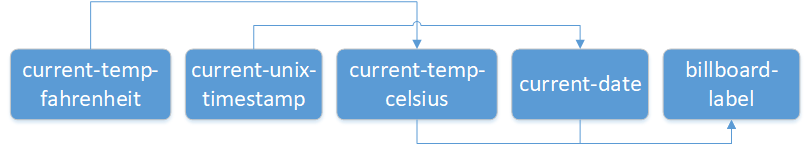
\includegraphics[width=\textwidth]{images/Language-FrDataflow-TopologicallySortedList.png}}
	\caption{The billboard as a topologically sorted list}
	\label{fig:language-frdataflow-topologically-sorted-list}
\end{figure}

\subsubsection{The update loop}

To implement the update behavior, each signal has a boolean flag indicating if it is stale or not. 
Upon startup of the runtime, FrDataFlow initializes a never ending update loop which loops over the topologically sorted list (as shown in figure \ref{fig:language-frdataflow-topologically-sorted-list}), skipping any signals which are not stale. 
If it encounters a stale signal, the lambda function that was provided during the creation of the signal will be called with the latest values of the parent signals. The signal is flagged as no longer being stale, and its direct children are flagged as stale immediately. Take for example an update of the current temperature. We start with a situation where the current date and temperature are already known and shown on the billboard, so the state of the signal graph looks like what is shown in figure \ref{fig:language-frdataflow-1}. 
Note that built in signals in FrDataFlow do not have a staleness flag, because they are kept up to date in separate runtime loops. 

\begin{figure}[h]
	\centerline{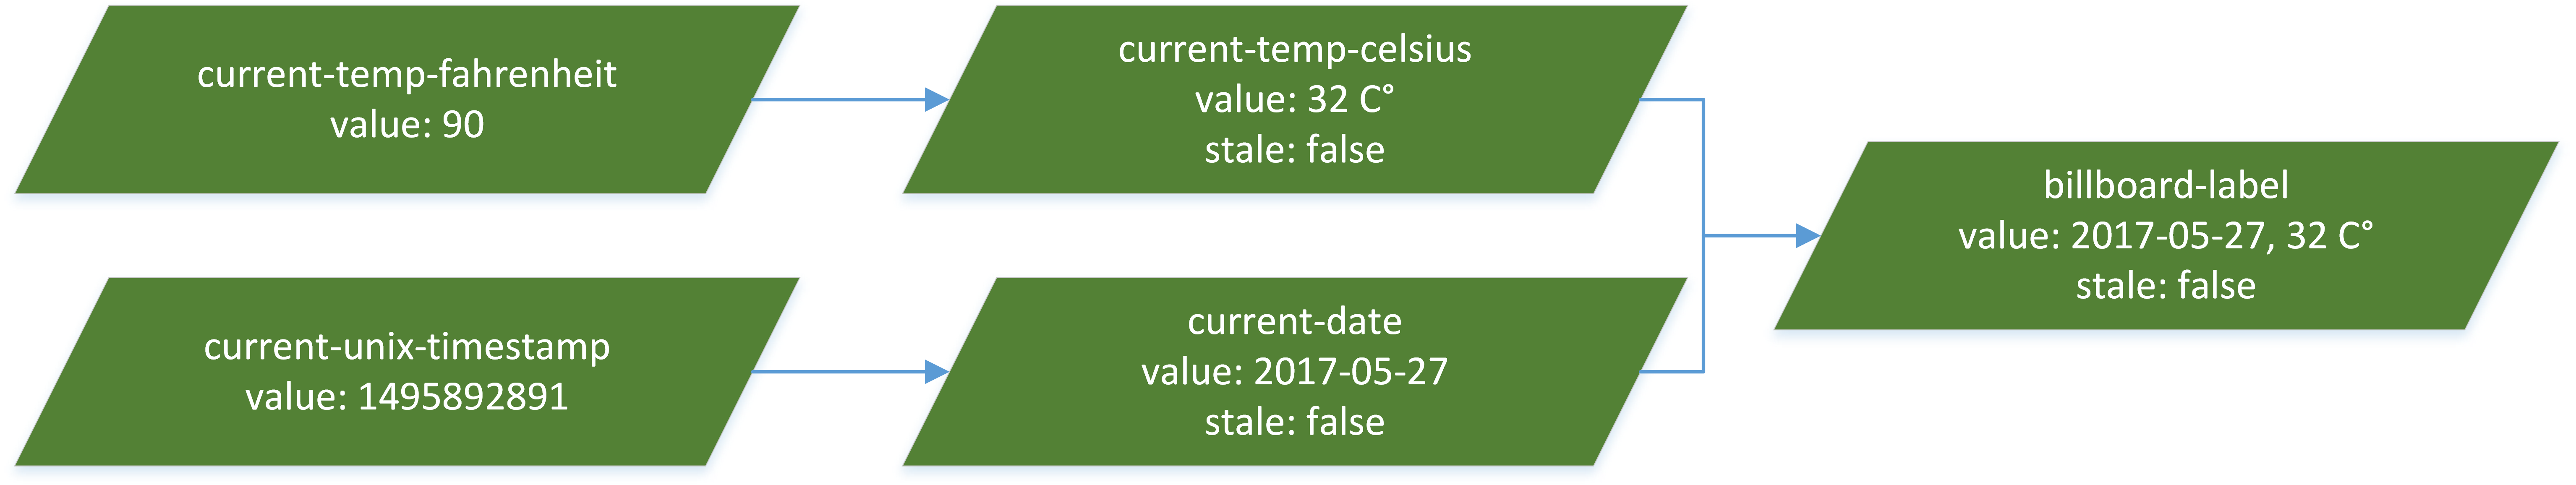
\includegraphics[width=\textwidth]{images/language-frdataflow-1.png}}
	\caption{The initial state of the billboard}
	\label{fig:language-frdataflow-1}
\end{figure}

When the new temperature is observed, the direct children of \textit{current-temp-fahrenheit} are flagged as stale, as shown in figure \ref{fig:language-frdataflow-2}.

\begin{figure}[h]
	\centerline{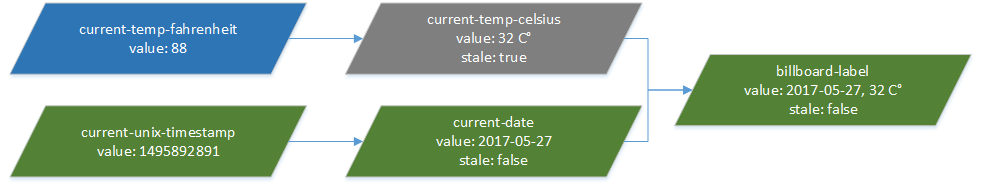
\includegraphics[width=\textwidth]{images/language-frdataflow-2.png}}
	\caption{A new temperature is emitted by current-temp-fahrenheit}
	\label{fig:language-frdataflow-2}
\end{figure}

The update loop sees that the signal has gone stale, recalculates what its value should be using the value of \textit{current-temp-fahrenheit} and removes the stale flag when its work is done.
However, it also immediately flags \textit{billboard-label} as stale, because it is registered as a child of \textit{current-temp-celsius}, as shown in figure \ref{fig:language-frdataflow-3}.

\begin{figure}[h]
	\centerline{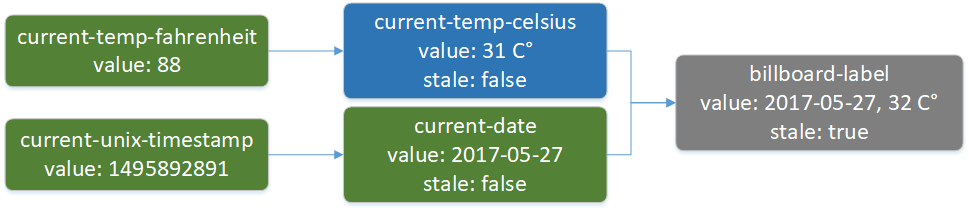
\includegraphics[width=\textwidth]{images/language-frdataflow-3.png}}
	\caption{current-temp-celsius gets recalculated}
	\label{fig:language-frdataflow-3}
\end{figure}

When the update loop moves further down the topologically sorted list, it sees that \textit{billboard-label} is also stale now. It grabs the latest values from \textit{current-temp-celsius} and \textit{current-date} and calls the lambda again that was used to create \textit{billboard-label}, removing the stale flag when it is done. The final result is shown in figure \ref{fig:language-frdataflow-4}. 
At this point, the update loop starts over again, waiting until another built in signal produces a new value. 

\begin{figure}[h]
	\centerline{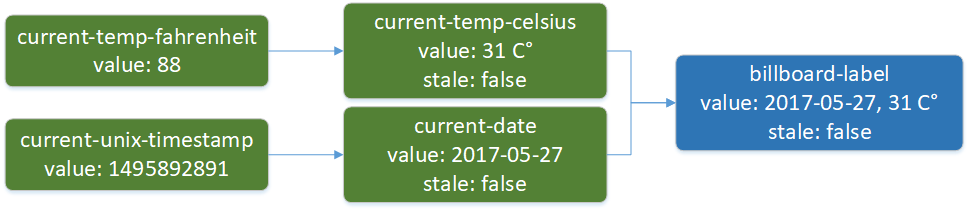
\includegraphics[width=\textwidth]{images/language-frdataflow-4.png}}
	\caption{billboard-label gets recalculated}
	\label{fig:language-frdataflow-4}
\end{figure}

\section{Conclusion}

In this chapter the reactive language FrDataFlow was presented with samples and diagrams of its implementation.
It is built as a metacircular evaluator that takes a core subset of the Racket language and extends it with some reactive concepts. FrDataFlow evaluates these expressions in a simulated runtime that forwards statements to the real underlying Racket implementation. 

This language can be used to model reactive data flows and provides a built in update loop to manage the data dependencies between signals. It does this by intelligently looping over the signals while being aware of the dependencies between them. New signals can be created by deriving from other signals and a lift function which produces a single value based on the values of the parent signals.